% Options for packages loaded elsewhere
\PassOptionsToPackage{unicode}{hyperref}
\PassOptionsToPackage{hyphens}{url}
\PassOptionsToPackage{dvipsnames,svgnames,x11names}{xcolor}
%
\documentclass[
  a4paper,
  DIV=11,
  numbers=noendperiod]{scrartcl}

\usepackage{amsmath,amssymb}
\usepackage{setspace}
\usepackage{iftex}
\ifPDFTeX
  \usepackage[T1]{fontenc}
  \usepackage[utf8]{inputenc}
  \usepackage{textcomp} % provide euro and other symbols
\else % if luatex or xetex
  \usepackage{unicode-math}
  \defaultfontfeatures{Scale=MatchLowercase}
  \defaultfontfeatures[\rmfamily]{Ligatures=TeX,Scale=1}
\fi
\usepackage{lmodern}
\ifPDFTeX\else  
    % xetex/luatex font selection
\fi
% Use upquote if available, for straight quotes in verbatim environments
\IfFileExists{upquote.sty}{\usepackage{upquote}}{}
\IfFileExists{microtype.sty}{% use microtype if available
  \usepackage[]{microtype}
  \UseMicrotypeSet[protrusion]{basicmath} % disable protrusion for tt fonts
}{}
\makeatletter
\@ifundefined{KOMAClassName}{% if non-KOMA class
  \IfFileExists{parskip.sty}{%
    \usepackage{parskip}
  }{% else
    \setlength{\parindent}{0pt}
    \setlength{\parskip}{6pt plus 2pt minus 1pt}}
}{% if KOMA class
  \KOMAoptions{parskip=half}}
\makeatother
\usepackage{xcolor}
\usepackage[headheight = 0 in,top = 1in,left = 0.8in,right =
0.8in,heightrounded]{geometry}
\setlength{\emergencystretch}{3em} % prevent overfull lines
\setcounter{secnumdepth}{-\maxdimen} % remove section numbering
% Make \paragraph and \subparagraph free-standing
\ifx\paragraph\undefined\else
  \let\oldparagraph\paragraph
  \renewcommand{\paragraph}[1]{\oldparagraph{#1}\mbox{}}
\fi
\ifx\subparagraph\undefined\else
  \let\oldsubparagraph\subparagraph
  \renewcommand{\subparagraph}[1]{\oldsubparagraph{#1}\mbox{}}
\fi


\providecommand{\tightlist}{%
  \setlength{\itemsep}{0pt}\setlength{\parskip}{0pt}}\usepackage{longtable,booktabs,array}
\usepackage{calc} % for calculating minipage widths
% Correct order of tables after \paragraph or \subparagraph
\usepackage{etoolbox}
\makeatletter
\patchcmd\longtable{\par}{\if@noskipsec\mbox{}\fi\par}{}{}
\makeatother
% Allow footnotes in longtable head/foot
\IfFileExists{footnotehyper.sty}{\usepackage{footnotehyper}}{\usepackage{footnote}}
\makesavenoteenv{longtable}
\usepackage{graphicx}
\makeatletter
\def\maxwidth{\ifdim\Gin@nat@width>\linewidth\linewidth\else\Gin@nat@width\fi}
\def\maxheight{\ifdim\Gin@nat@height>\textheight\textheight\else\Gin@nat@height\fi}
\makeatother
% Scale images if necessary, so that they will not overflow the page
% margins by default, and it is still possible to overwrite the defaults
% using explicit options in \includegraphics[width, height, ...]{}
\setkeys{Gin}{width=\maxwidth,height=\maxheight,keepaspectratio}
% Set default figure placement to htbp
\makeatletter
\def\fps@figure{htbp}
\makeatother

\usepackage{booktabs}
\usepackage{longtable}
\usepackage{array}
\usepackage{multirow}
\usepackage{wrapfig}
\usepackage{float}
\usepackage{colortbl}
\usepackage{pdflscape}
\usepackage{tabu}
\usepackage{threeparttable}
\usepackage{threeparttablex}
\usepackage[normalem]{ulem}
\usepackage{makecell}
\usepackage{xcolor}
\KOMAoption{captions}{tableheading}
\makeatletter
\@ifpackageloaded{caption}{}{\usepackage{caption}}
\AtBeginDocument{%
\ifdefined\contentsname
  \renewcommand*\contentsname{Table of contents}
\else
  \newcommand\contentsname{Table of contents}
\fi
\ifdefined\listfigurename
  \renewcommand*\listfigurename{List of Figures}
\else
  \newcommand\listfigurename{List of Figures}
\fi
\ifdefined\listtablename
  \renewcommand*\listtablename{List of Tables}
\else
  \newcommand\listtablename{List of Tables}
\fi
\ifdefined\figurename
  \renewcommand*\figurename{Figure}
\else
  \newcommand\figurename{Figure}
\fi
\ifdefined\tablename
  \renewcommand*\tablename{Table}
\else
  \newcommand\tablename{Table}
\fi
}
\@ifpackageloaded{float}{}{\usepackage{float}}
\floatstyle{ruled}
\@ifundefined{c@chapter}{\newfloat{codelisting}{h}{lop}}{\newfloat{codelisting}{h}{lop}[chapter]}
\floatname{codelisting}{Listing}
\newcommand*\listoflistings{\listof{codelisting}{List of Listings}}
\makeatother
\makeatletter
\makeatother
\makeatletter
\@ifpackageloaded{caption}{}{\usepackage{caption}}
\@ifpackageloaded{subcaption}{}{\usepackage{subcaption}}
\makeatother
\ifLuaTeX
  \usepackage{selnolig}  % disable illegal ligatures
\fi
\usepackage{bookmark}

\IfFileExists{xurl.sty}{\usepackage{xurl}}{} % add URL line breaks if available
\urlstyle{same} % disable monospaced font for URLs
\hypersetup{
  pdftitle={IO2 PS2 Bresnahan and Reiss (1991)},
  pdfauthor={Carlos T. Estrada Arzamendi},
  colorlinks=true,
  linkcolor={blue},
  filecolor={Maroon},
  citecolor={Blue},
  urlcolor={Blue},
  pdfcreator={LaTeX via pandoc}}

\title{IO2 PS2 Bresnahan and Reiss (1991)}
\author{Carlos T. Estrada Arzamendi}
\date{March 26, 2024}

\begin{document}
\maketitle

\setstretch{1.25}
\section{Problem 1 :}\label{problem-1}

\begin{quote}
Reproduce the results for the tire dealers reported in Table 4 of the
paper. Note that Bresnahan and Reiss (1991) estimate the model imposing
the constraints \(\alpha_n \geq 0\) and \(\gamma_n \geq 0\). You should
impose the same constraints.
\end{quote}

\subsection{Reproducing Figure 2 to get to know the
data}\label{reproducing-figure-2-to-get-to-know-the-data}

\begin{figure}[H]

{\centering 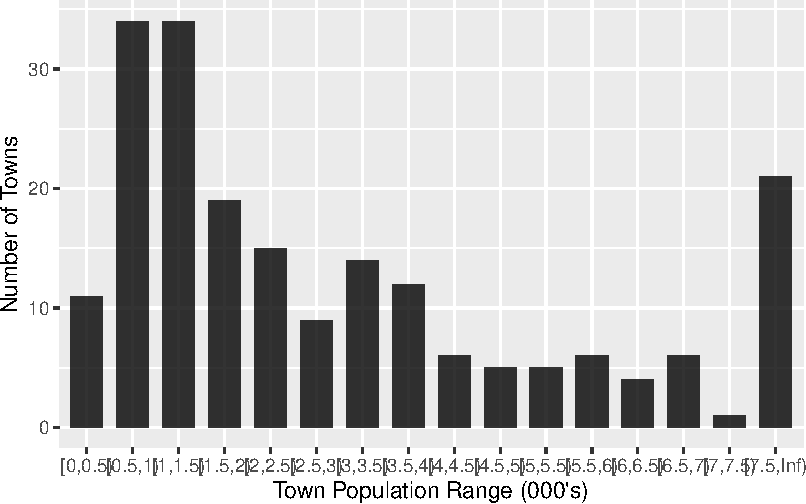
\includegraphics[width=0.76\textwidth,height=\textheight]{IO2_PS2_Estrada_files/figure-pdf/figure2-1.pdf}

}

\caption{Number of towns by town population}

\end{figure}%

\newpage

\subsection{Reproducing Table 3 to get to know the
data}\label{reproducing-table-3-to-get-to-know-the-data}

\begin{longtable}[]{@{}
  >{\raggedright\arraybackslash}p{(\columnwidth - 14\tabcolsep) * \real{0.0897}}
  >{\raggedleft\arraybackslash}p{(\columnwidth - 14\tabcolsep) * \real{0.1026}}
  >{\raggedleft\arraybackslash}p{(\columnwidth - 14\tabcolsep) * \real{0.1795}}
  >{\raggedleft\arraybackslash}p{(\columnwidth - 14\tabcolsep) * \real{0.1282}}
  >{\raggedleft\arraybackslash}p{(\columnwidth - 14\tabcolsep) * \real{0.1282}}
  >{\raggedleft\arraybackslash}p{(\columnwidth - 14\tabcolsep) * \real{0.1154}}
  >{\raggedleft\arraybackslash}p{(\columnwidth - 14\tabcolsep) * \real{0.1282}}
  >{\raggedleft\arraybackslash}p{(\columnwidth - 14\tabcolsep) * \real{0.1282}}@{}}
\caption{Replication of Table 3}\tabularnewline
\toprule\noalign{}
\begin{minipage}[b]{\linewidth}\raggedright
\end{minipage} & \begin{minipage}[b]{\linewidth}\raggedleft
Unique
\end{minipage} & \begin{minipage}[b]{\linewidth}\raggedleft
Missing Pct.
\end{minipage} & \begin{minipage}[b]{\linewidth}\raggedleft
Mean
\end{minipage} & \begin{minipage}[b]{\linewidth}\raggedleft
SD
\end{minipage} & \begin{minipage}[b]{\linewidth}\raggedleft
Min
\end{minipage} & \begin{minipage}[b]{\linewidth}\raggedleft
Median
\end{minipage} & \begin{minipage}[b]{\linewidth}\raggedleft
Max
\end{minipage} \\
\midrule\noalign{}
\endfirsthead
\toprule\noalign{}
\begin{minipage}[b]{\linewidth}\raggedright
\end{minipage} & \begin{minipage}[b]{\linewidth}\raggedleft
Unique
\end{minipage} & \begin{minipage}[b]{\linewidth}\raggedleft
Missing Pct.
\end{minipage} & \begin{minipage}[b]{\linewidth}\raggedleft
Mean
\end{minipage} & \begin{minipage}[b]{\linewidth}\raggedleft
SD
\end{minipage} & \begin{minipage}[b]{\linewidth}\raggedleft
Min
\end{minipage} & \begin{minipage}[b]{\linewidth}\raggedleft
Median
\end{minipage} & \begin{minipage}[b]{\linewidth}\raggedleft
Max
\end{minipage} \\
\midrule\noalign{}
\endhead
\bottomrule\noalign{}
\endlastfoot
ID & 202 & 0 & 328090.8 & 143299.0 & 40013.0 & 320014.0 & 560045.0 \\
TIRE & 14 & 0 & 2.6 & 2.6 & 0.0 & 2.0 & 13.0 \\
TPOP & 195 & 0 & 3.7 & 5.4 & 0.1 & 2.1 & 45.1 \\
NGRW & 58 & 0 & -0.1 & 0.1 & -1.3 & 0.0 & 0.0 \\
PGRW & 119 & 0 & 0.5 & 1.1 & 0.0 & 0.1 & 7.2 \\
OCTY & 160 & 0 & 0.3 & 0.7 & 0.0 & 0.2 & 8.4 \\
OPOP & 178 & 0 & 0.4 & 0.7 & 0.0 & 0.1 & 5.8 \\
LANDV & 166 & 0 & 0.3 & 0.2 & 0.1 & 0.2 & 1.6 \\
ELD & 198 & 0 & 0.1 & 0.0 & 0.0 & 0.1 & 0.3 \\
FFRAC & 174 & 0 & 0.7 & 0.4 & 0.0 & 0.8 & 1.3 \\
PINC & 191 & 0 & 5.9 & 1.1 & 3.2 & 5.9 & 10.5 \\
LNHDD & 62 & 0 & 8.6 & 0.5 & 6.8 & 8.7 & 9.2 \\
\end{longtable}

\subsection{Main Task: Replication of Table
4}\label{main-task-replication-of-table-4}

I found that the results obtained from the optimization are highly
dependent on the starting values:

\begin{enumerate}
\def\labelenumi{\arabic{enumi}.}
\item
  Starting far from the results found from BR1991, the optimizer finds a
  set of parameters that has a lower Likelihood than the true parameters
  (using the same likelihood function), despite the BR1991 parameters
  being in the support.
\item
  Starting a the vector of estimates shown in BR19991, I get results
  that appear correct.
\end{enumerate}

This take me to believe the R optimizer I am using is the root to the
discrepancy.

\begin{longtable}[]{@{}
  >{\raggedright\arraybackslash}p{(\columnwidth - 6\tabcolsep) * \real{0.1974}}
  >{\raggedleft\arraybackslash}p{(\columnwidth - 6\tabcolsep) * \real{0.2763}}
  >{\raggedleft\arraybackslash}p{(\columnwidth - 6\tabcolsep) * \real{0.3158}}
  >{\raggedleft\arraybackslash}p{(\columnwidth - 6\tabcolsep) * \real{0.2105}}@{}}
\caption{MLE Parameter Estimates}\tabularnewline
\toprule\noalign{}
\begin{minipage}[b]{\linewidth}\raggedright
Parameter
\end{minipage} & \begin{minipage}[b]{\linewidth}\raggedleft
Estimate (Far Start)
\end{minipage} & \begin{minipage}[b]{\linewidth}\raggedleft
Estimate (BR1991 Start)
\end{minipage} & \begin{minipage}[b]{\linewidth}\raggedleft
BR1991 Estimate
\end{minipage} \\
\midrule\noalign{}
\endfirsthead
\toprule\noalign{}
\begin{minipage}[b]{\linewidth}\raggedright
Parameter
\end{minipage} & \begin{minipage}[b]{\linewidth}\raggedleft
Estimate (Far Start)
\end{minipage} & \begin{minipage}[b]{\linewidth}\raggedleft
Estimate (BR1991 Start)
\end{minipage} & \begin{minipage}[b]{\linewidth}\raggedleft
BR1991 Estimate
\end{minipage} \\
\midrule\noalign{}
\endhead
\bottomrule\noalign{}
\endlastfoot
lambda1 & -0.57227 & -0.53072 & -0.530 \\
lambda2 & 0.60978 & 2.25000 & 2.250 \\
lambda3 & 0.61129 & 0.33997 & 0.340 \\
lambda4 & 0.08496 & 0.22938 & 0.230 \\
beta1 & -0.25757 & -0.49006 & -0.490 \\
beta2 & -0.01488 & -0.03051 & -0.030 \\
beta3 & -0.03657 & 0.00401 & 0.004 \\
beta4 & -0.01784 & -0.02064 & -0.020 \\
alpha1 & 0.95743 & 0.85959 & 0.860 \\
alpha2 & 0.00032 & 0.03294 & 0.030 \\
alpha3 & 0.06695 & 0.15162 & 0.150 \\
alpha4 & 0.00351 & 0.00000 & 0.000 \\
alpha5 & 0.08293 & 0.08057 & 0.080 \\
gamma1 & 0.42810 & 0.52970 & 0.530 \\
gamma2 & 0.76995 & 0.75979 & 0.760 \\
gamma3 & 0.64751 & 0.46127 & 0.460 \\
gamma4 & 0.55471 & 0.59872 & 0.600 \\
gamma5 & 0.10361 & 0.12015 & 0.120 \\
gamma\_L & -0.82611 & -0.73968 & -0.740 \\
Log Likelihood & -264.76586 & -263.09143 & -263.158 \\
\end{longtable}



\end{document}
